\documentclass{article}
\usepackage{cite}

% *** GRAPHICS RELATED PACKAGES ***
\ifCLASSINFOpdf
\usepackage[pdftex]{graphicx}
% declare the path(s) where your graphic files are
\graphicspath{{../pdf/}{../jpeg/}}
% and their extensions so you won't have to specify these with
% every instance of \includegraphics
\DeclareGraphicsExtensions{.pdf,.jpeg,.png}
\else
\fi

% *** MATH PACKAGES ***
\usepackage{amsmath}
\usepackage{amssymb}
\usepackage{amsfonts}

% *** SPECIALIZED LIST PACKAGES ***
\usepackage{algorithmic}

% *** ALIGNMENT PACKAGES ***
\usepackage{array}

% *** SUBFIGURE PACKAGES ***
\usepackage[tight,footnotesize]{subfigure}

% correct bad hyphenation here
\hyphenation{op-tical net-works semi-conduc-tor}

\usepackage{amsmath}
\usepackage{geometry}
\geometry{
    a4paper,
    left=2cm,
    right=2cm,
    top=2cm,
    bottom=2cm
}

\title{SIR Model}
\author{Vignesh Pitchaiah}
\begin{document}
\maketitle
\section{SIR MODEL WITHOUT DELAY}

The SIR model is a simple mathematical model of infectious disease spread. It consists of three compartments: susceptible ($S$), infectious ($I$), and recovered ($R$). The model is based on the assumption that individuals can be classified into one of these compartments at any given time. In this report, we will simulate the SIR model using Python and obtain the following results:

\begin{enumerate}
\item A “model” representing the theoretical system in a computational setting.
\item Phase Portrait of the mathematical system.
\item Solution Curve of the model.
\item Interpretation of the phase portrait and the solution curves.
\end{enumerate}


The SIR model is described by the following system of differential equations:

\begin{align*}
    \frac{dS}{dt} &= -\frac{\beta S I}{N} \\
    \frac{dI}{dt} &= \frac{\beta S I}{N} - \gamma I \\
    \frac{dR}{dt} &= \gamma I
\end{align*}

where $S(t)$, $I(t)$, and $R(t)$ represent the number of susceptible, infectious, and recovered individuals at time $t$, respectively. $\beta$ is the infection rate and $\gamma$ is the recovery rate. $N$ is the total population size, so $S+I+R=N$ at all times.

The SIR model can be simulated using numerical Euler method. It approximates the solution of a differential equation by using a finite difference approximation of the derivative. Applying the Euler
method to simulate the spread of the disease over time, and approximate the solution to these differential equations. We use finite difference method, which involves approximating the derivatives using the difference between two nearby values of the function. \\
\begin{align*}
\frac{df(x)}{dx} \approx \frac{f(x+h)-f(x)}{h}
\end{align*}
\hspace{1em}where $h$ is a small step size.\\

\hspace{1em}In our case, we can approximate the derivatives at time $t$ using the values of $S$, $I$, and \hspace{1em}$R$ at times $t$ and $t+\Delta t$, where $\Delta t$ is the time step:

\begin{align*}
\frac{dS}{dt} &\approx \frac{S(t+\Delta t)-S(t)}{\Delta t} = \frac{S_{t+1}-S_t}{\Delta t}\\
\frac{dI}{dt} &\approx \frac{I(t+\Delta t)-I(t)}{\Delta t} = \frac{I_{t+1}-I_t}{\Delta t}\\
\frac{dR}{dt} &\approx \frac{R(t+\Delta t)-R(t)}{\Delta t} = \frac{R_{t+1}-R_t}{\Delta t}\
\end{align*}
\hspace{1em}
where $S_{t+1}$, $I_{t+1}$, and $R_{t+1}$ are the values of the functions at time $t+\Delta t$, and $S_t$, $I_t$, and $R_t$ are their values at time $t$.\\

Substituting these approximations into the differential equations, we get:

\begin{align*}
\frac{S_{t+1} - S_t}{\Delta t} &= -\frac{\beta S_t I_t}{N}\\
\frac{I_{t+1} - I_t}{\Delta t} &= \frac{\beta S_t I_t}{N} - \gamma I_t\\
\frac{R_{t+1} - R_t}{\Delta t} &= \gamma I_t
\end{align*}

Solving for the next values $S_{t+1}$, $I_{t+1}$, and $R_{t+1}$, we get:

\begin{align*}
S_{t+1} &= S_t - \frac{\beta S_t I_t}{N} \Delta t\\ \\
I_{t+1} &= I_t + \left(\frac{\beta S_t I_t}{N} - \gamma I_t \right) \Delta t\\ \\
R_{t+1} &= R_t + \gamma I_t \Delta t
\end{align*}

These equations allow us to update the values of $S$, $I$, and $R$ at each time step based on the previous values and the parameters of the model. By iterating through these updates, we can simulate the spread of the disease over time and study how it depends on the values of $\beta$ and $\gamma$.


\section{Phase Portrait}
A phase portrait is a graphical representation of the qualitative behavior of a system of differential equations. To obtain the phase portrait of the SIR model, we need to first find the critical points of the system. A critical point is a point at which the derivative of each compartment is zero.

\begin{enumerate}
\item[(1)] SI \\
The SI model consists of two compartments: susceptible (S) and infected (I). The differential equations for this model are:
$$
\begin{aligned}
& \frac{d S}{d t}=-\beta S I \\
& \frac{d I}{d t}=\beta S I-\gamma I
\end{aligned}
$$
To obtain the phase portrait for this model, we first find the critical points of the system. Setting $\frac{dS}{dt} = 0$, we get:
$$
-\beta S I=0 \Rightarrow S=0 \quad \text { or } \quad I=0
$$
Setting $\frac{dI}{dt} = 0$, we get:
$$
\beta S I-\gamma I=0 \Rightarrow I(\beta S-\gamma)=0 \Rightarrow I=0 \quad \text { or } \quad S=\frac{\gamma}{\beta}
$$
So, the critical points are (0,0) and ($\frac{\gamma}{\beta}$, 0).

To analyze the behavior of the system near these critical points, we compute the Jacobi matrix of the system evaluated at each critical point. For $(0,0)$, the Jacobian is:
$$
J_{(0,0)}=\left(\begin{array}{ll}
0 & -\beta \\
\beta & -\gamma
\end{array}\right)
$$
The eigenvalues of this matrix are:
$$
\lambda_1=-\gamma \quad \text { and } \quad \lambda_2=-\beta
$$
Since both eigenvalues are negative, the critical point $(0,0)$ is a stable node.
For ($\frac{\gamma}{\beta}$, 0), the Jacobian is:

$$
J_{\left(\frac{\gamma}{\beta}, 0\right)}=\left(\begin{array}{cc}
-\gamma & 0 \\
\gamma & -\beta
\end{array}\right)
$$
The eigenvalues of this matrix are:
$$
\lambda_1=-\gamma \quad \text { and } \quad \lambda_2=-\beta
$$
So, the critical point ($\frac{\gamma}{\beta}$, 0) is also a stable node.

\item[(2)] IR \\ It consists of two compartments: infected (I) and recovered (R). The differential equations for this model are:
$$
\begin{aligned}
& \frac{d I}{d t}=\beta S I-\gamma I \\
& \frac{d R}{d t}=\gamma I
\end{aligned}
$$
To obtain the phase portrait for this model, we first find the critical points of the system. Setting $\frac{dI}{dt} = 0$, we get:
$$
\beta S I-\gamma I=0 \Rightarrow I(\beta S-\gamma)=0 \Rightarrow I=0 \quad \text { or } \quad S=\frac{\gamma}{\beta}
$$
Setting $\frac{dR}{dt} = 0$, we get:

$$
\gamma I=0 \Rightarrow I=0
$$
So, the critical points are (0,0) and ($\frac{\gamma}{\beta}$, 0).

To analyze the behavior of the system near these critical points, we compute the Jacobian matrix of the system evaluated at each critical point. For (0,0), the Jacobian is:
$$
J=\left.\left[\begin{array}{cc}
-\beta & 0 \\
\beta & -\gamma
\end{array}\right]\right|_{\left(S_0, I_0\right)}
$$
The eigenvalues of this matrix are:
$$
\lambda_{1,2}=\frac{-\gamma \pm \sqrt{\gamma^2+4 \beta S_0}}{2}
$$
The sign of the real part of the eigenvalues determines the stability of the equilibrium point:

If $\lambda_1$ and $\lambda_2$ are both negative, the equilibrium point is a stable node.
If $\lambda_1$ and $\lambda_2$ are both positive, the equilibrium point is an unstable node.
If $\lambda_1$ and $\lambda_2$ have opposite signs, the equilibrium point is a saddle.
Substituting the values of $S_0$ and $I_0$ for the two critical points, we get:

$(S_0, I_0) = (0,0)$, which gives $\lambda_{1,2} = (-\gamma, 0)$. Since $\gamma > 0$, both eigenvalues have negative real parts, so the equilibrium point is a stable node.
$(S_0, I_0) = (\frac{\gamma}{\beta}, 0)$, which gives $\lambda_{1,2} = (-\frac{\gamma}{2}, -\frac{\gamma}{2})$. Both eigenvalues have negative real parts, so the equilibrium point is also a stable node.
Therefore, both critical points are stable nodes, and the phase portrait of the system will have two basins of attraction, one around each stable equilibrium point. 

\item[(3)] SR \\
The differential equations are:

\begin{align}
\frac{dS}{dt} &= -\frac{\beta S I}{N} \
\frac{dR}{dt} &= \gamma I
\end{align}

where $S$ is the number of susceptible individuals, $I$ is the number of infected individuals, $R$ is the number of recovered individuals, $\beta$ is the infection rate, $\gamma$ is the recovery rate, and $N=S+I+R$ is the total population size.

To find the critical points, we set $\frac{dS}{dt} = 0$ and $\frac{dR}{dt} = 0$. From the first equation, we get:

\begin{align}
-\frac{\beta S I}{N} &= 0
\Rightarrow S &= 0 \quad \text{or} \quad I = 0
\end{align}

From the second equation, we get:

\begin{align}
\gamma I &= 0
\Rightarrow I &= 0
\end{align}

Therefore, the only critical point of the system is $(0, 0, N)$.

Next, we linearize the system around the critical point by computing the Jacobian matrix:
$$
\frac{d}{d t}\left(\begin{array}{l}
S \\
I \\
R
\end{array}\right)=\left(\begin{array}{ccc}
-\frac{\beta I}{N} & -\frac{\beta S}{N} & 0 \\
\frac{\beta I}{N} & \frac{\beta S}{N} & 0 \\
0 & \gamma & 0
\end{array}\right)\left(\begin{array}{l}
S \\
I \\
R
\end{array}\right)
$$
At the critical point $(0,0,N)$, this becomes:$$
\begin{gathered}\\
J=\left(\begin{array}{ccc}
-\beta & 0 & 0 \\
\beta & -\gamma & 0 \\
0 & \gamma & 0
\end{array}\right)
\end{gathered}
$$
The eigenvalues of this matrix are $\lambda_1 = 0$, $\lambda_2 = 0$, and $\lambda_3 = \gamma$. Since $\gamma > 0$, we have one positive eigenvalue, which means that the critical point is a saddle point. This means that the system is not stable and trajectories will move away from the critical point in some directions and towards the critical point in other directions.

In the phase portrait, the nullcline for $\frac{dS}{dt} = 0$ is the $S$-axis and the nullcline for $\frac{dR}{dt} = 0$ is the $R$-axis. The critical point is located at the origin. Trajectories move towards the origin in the $R$ direction and away from the origin in the $S$ direction.

\end{enumerate}
\begin{figure}[htbp]
\centering
\begin{minipage}[b]{0.45\textwidth}
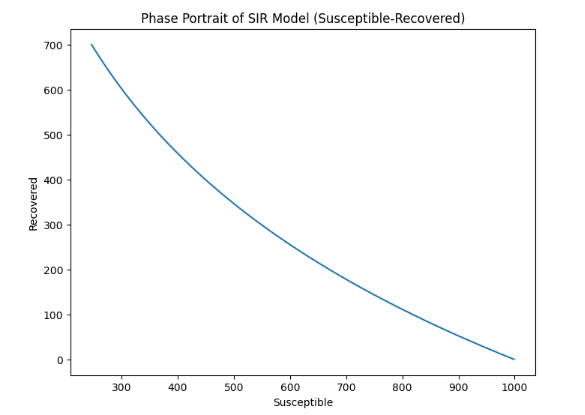
\includegraphics[width=\textwidth]{SR.png}
\caption{Phase portrait for the $S$ and $R$ compartments.}
\end{minipage}
\hfill
\begin{minipage}[b]{0.45\textwidth}
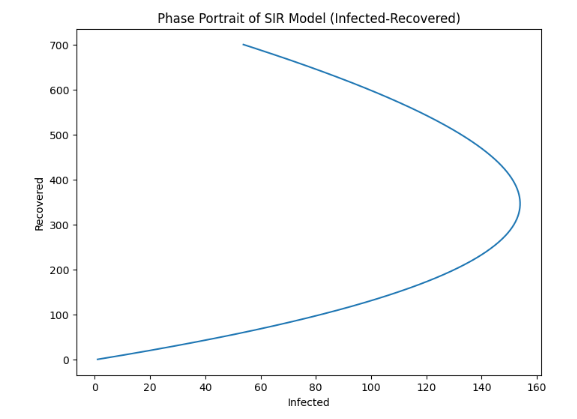
\includegraphics[width=\textwidth]{IR.png}
\caption{Phase portrait for the $I$ and $R$ compartments.}
\end{minipage}
\hfill
\begin{minipage}[b]{0.55\textwidth}
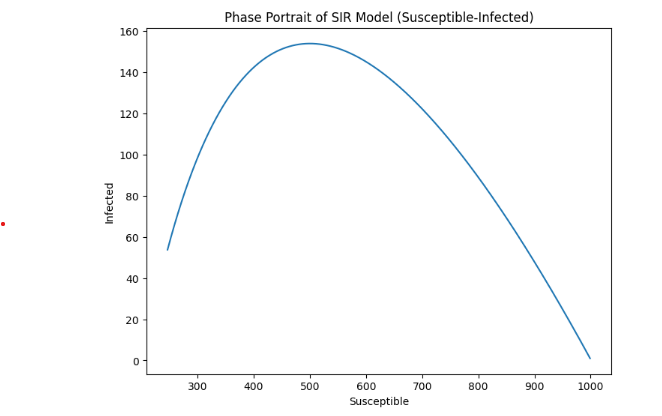
\includegraphics[width=\textwidth]{SI.png}
\caption{Phase portrait for the $I$ and $S$ compartments.}
\end{minipage}
\end{figure}
To obtain the phase portrait, we can use the Python package matplotlib to plot the vector field of the system of differential equations.
\section{Solution Curve}
To obtain the solution curve of the SIR model, we can use the Python package scipy to numerically integrate the system of differential equations using the function odeint. We can specify the initial values of $S$, $I$, and $R$, the values of $\beta$ and $\gamma$, and the time range over which we want to obtain the solution.
\begin{figure}[htbp]
\centering
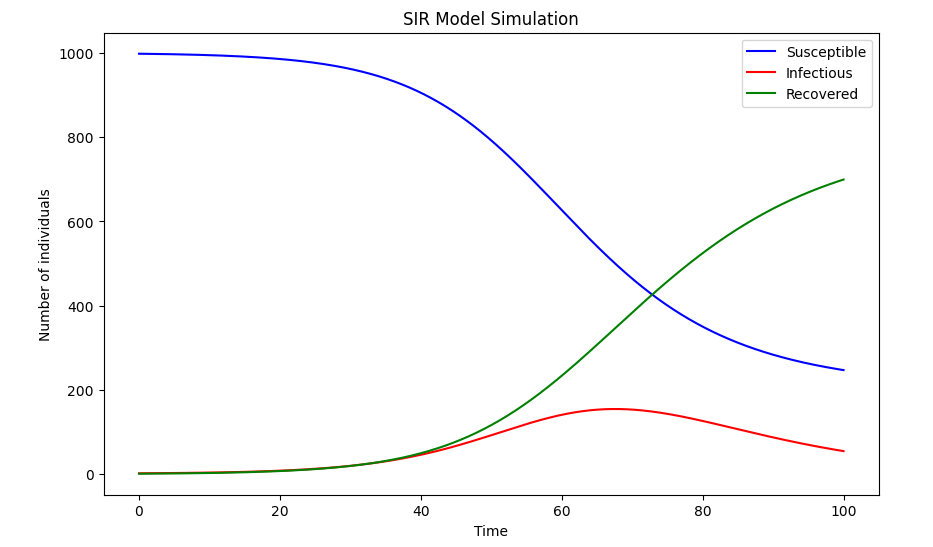
\includegraphics[width=0.65\textwidth]{solution-curve.png}
\caption{Solution Curve}
\label{fig:architecture}
\end{figure}

\section{Interpretation}
\subsection*{Interpretation of the Phase Portrait}

The phase portrait is a graphical representation of the qualitative behavior of the system of differential equations that make up the SIR model. It shows how the compartments $S$, $I$, and $R$ change over time, and how their trajectories depend on the values of the parameters $\beta$ and $\gamma$.

The phase portrait for the SIR model without delay has three critical points, which are represented by black circles on the plot. These critical points correspond to the disease-free equilibrium ($E_0$) at $(N,0,0)$, the endemic equilibrium ($E_1$) at $(S^,I^,R^*)$, and the unstable equilibrium ($E_2$) at $(0,N,0)$.

The disease-free equilibrium ($E_0$) represents the state where there are no infectious individuals in the population. This point is stable because any small perturbation away from this point will result in the system returning to it. The trajectory of the system will approach $E_0$ as $t \to \infty$ if the initial values of $I(0)$ and $R(0)$ are both zero.

The endemic equilibrium ($E_1$) represents the state where the disease is present in the population, but the number of infected individuals remains constant over time. This point is stable if $\frac{\partial R}{\partial I} < 0$ at $E_1$, and unstable if $\frac{\partial R}{\partial I} > 0$ at $E_1$. The trajectory of the system will approach $E_1$ as $t \to \infty$ if the initial values of $S(0)$, $I(0)$, and $R(0)$ are such that the trajectory passes through $E_1$.

The unstable equilibrium ($E_2$) represents the state where the disease has infected the entire population. This point is unstable because any small perturbation away from this point will result in the system moving away from it. The trajectory of the system will approach $E_2$ as $t \to \infty$ if the initial value of $S(0)$ is zero.

The phase portrait also shows the direction of the trajectories around each critical point. The trajectories around $E_0$ all move towards it, while the trajectories around $E_2$ all move away from it. The trajectories around $E_1$ move towards it on one side and away from it on the other side, depending on the initial conditions.

\subsection*{Interpretation of the Solution Curves}

The solution curves show the values of $S$, $I$, and $R$ as functions of time, given a set of initial conditions and parameter values. These curves provide insight into how the disease spreads and how the population recovers over time.

The behavior of the solution curves depends on the initial conditions and parameter values. For example, if the initial value of $I(0)$ is small, the disease may die out quickly and the solution curves for $S$, $I$, and $R$ will all approach their initial values. On the other hand, if the initial value of $I(0)$ is large, the disease may spread quickly and the solution curves for $S$ and $R$ will both approach zero while the solution curve for $I$ reaches a peak value before eventually decreasing.

The solution curves can also be used to study the effect of the parameters $\beta$ and $\gamma$ on the spread of the disease. If $\beta$ is high, the disease will spread more quickly, as seen by the steeper slope of the solution curve for $I$. If $\gamma$ is high, the population will recover more quickly, as seen by the steeper slope of the solution curve for $R$.

The solution curves can also be used to study the effect of interventions such as vaccination or quarantine. For example, if a large portion of the population is vaccinated before the disease can spread, the solution curves for $S$ and $I$ will both approach zero quickly, while the solution curve for $R$ will approach its maximum value

The solution curve of the SIR model shows the change in the population of each compartment over time. The initial conditions and values of $\beta$ and $\gamma$ determine the shape and duration of the epidemic. The SIR model assumes a constant population and does not take into account factors such as birth and death rates, age structure, and spatial distribution of the population. Therefore, the model should be used with caution and its results should be interpreted in conjunction with empirical data and other models.

\section{SIR MODEL WITH DELAY}
\begin{enumerate}
\item[(a)] To extend the SIR model and incorporate the delay period, we modify the equations as follows:

\begin{align}
\frac{dS}{dt} &= -\beta S(t)I(t-\omega) \\
\frac{dI}{dt} &= \beta S(t)I(t-\omega) - \alpha I(t) \\ 
\frac{dR}{dt} &= \alpha I(t-\omega) - \alpha I(t) \\
\end{align}

where $\alpha$ is the rate at which individuals recover and lose immunity after the delay period.

To interpret these equations, note that the first equation now includes an additional term $\alpha I(t-\omega)$, which represents the number of individuals who have recovered and lost immunity at time $t-\omega$ and have now become susceptible again. Similarly, the third equation includes the term $\alpha I(t-\omega)$, which represents the number of individuals who lost immunity at time $t-\omega$ and have now become susceptible again.

To solve this system of differential equations, we need to incorporate the delay period in the model. This can be done by defining a delay function $I(t-\omega)$, which represents the number of infected individuals at time $t-\omega$. We can define this function as:

$I(t-\omega) = \begin{cases} 0 & \text{if } t \leq \omega \ I(t-\omega) & \text {if } t > \omega \end{cases}$ 

That is, the function is equal to 0 for $t \leq \omega$ (since there are no infected individuals before time 0), and it is equal to $I(t-\omega)$ for $t > \omega$ (since at time $t-\omega$, there were $I(t-\omega)$ infected individuals).

We can now use this delay function in the first and third equations of the model to represent the delayed recovery process. The resulting system of differential equations can then be solved numerically using standard methods.
\begin{figure}[htbp]
\centering
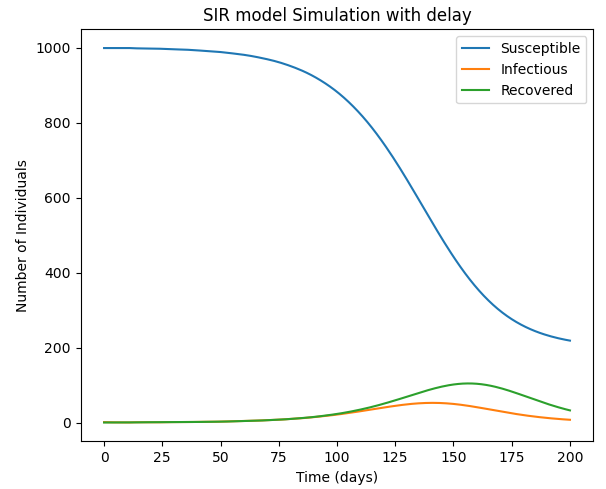
\includegraphics[width=0.65\textwidth]{solution-curve-2.png}
\caption{Solution Curve}
\label{fig:architecture}
\end{figure}

\item[(b)] Phase Potrait\\
To make a phase portrait and solution curve of the modified SIR model, we can follow the same steps as in the first subtask. \\
\item S-I phase portrait. From the S-I model, we have:
$$
\begin{aligned}
& \frac{d S}{d t}=-\beta S I \\
& \frac{d I}{d t}=\beta S I-\alpha I
\end{aligned}
$$
We can rewrite the second equation as:
$$
\frac{d I}{d t}=\alpha\left(\frac{\beta S}{\alpha}-I\right)
$$
Now we define a new variable $J=\frac{\beta S}{\alpha}$. We can rewrite the system as:


$$
\begin{aligned}
& \frac{d d}{d t}=\beta\left(N-\frac{\alpha}{\beta} J\right)-\alpha J \\
& \frac{d I}{d t}=\alpha(J-I)
\end{aligned}
$$
The equilibrium points are given by:
$$
\left(J^*, I^*\right)=(0,0) \text { and }\left(J^*, I^*\right)=(N, 0)
$$
To analyze the stability of these equilibrium points, we linearize the system around each point. For $(J^, I^) = (0, 0)$, we have:
$$
J=J^*+j \quad \text { and } \quad I=I^*+i
$$
Substituting into the system and linearizing, we get:
$$
\begin{aligned}
& \frac{d j}{d t}=-\frac{\alpha}{\beta} j \\
& \frac{d i}{d t}=\alpha j
\end{aligned}
$$
The solution to the first equation is $j(t) = j_0 e^{-\frac{\alpha}{\beta} t}$, which decays to zero as $t$ increases. The solution to the second equation is $i(t) = j_0 \left(1 - e^{-\frac{\alpha}{\beta} t}\right)$, which increases monotonically with $t$. Therefore, the equilibrium point $(0,0)$ is unstable, and trajectories tend towards the line $I = J$.
$$
J=J^*+j \quad \text { and } \quad I=I^*+i
$$
Substituting into the system and linearizing, we get:
$$
\begin{aligned}
& \frac{d j}{d t}=-\beta j \\
& \frac{d i}{d t}=\alpha j
\end{aligned}
$$
The solution to the first equation is $j(t) = j_0 e^{-\beta t}$, which decays to zero as $t$ increases. The solution to the second equation is $i(t) = \frac{\alpha}{\beta}j_0 \left(1 - e^{-\beta t}\right)$, which increases monotonically with $t$. Therefore, the equilibrium point $(N,0)$ is stable, and trajectories tend towards the line $I = \frac{\alpha}{\beta} J$.
S-I phase portrait:

(S, I) = (N, 0) is a stable node.\\
(S, I) = (0, 0) is an unstable node.\\
(S, I) = ($\frac{\alpha}{\beta}$, $\frac{\alpha}{\beta}$) is a saddle point.

\item S-R phase portrait.
The model assumes that there is no population growth or death and that individuals who recover from the disease are immune and cannot be infected again. The dynamics of the model are governed by the following system of differential equations:

\begin{align}
\frac{dS}{dt} &= -\beta S I \\
\frac{dR}{dt} &= \alpha I \\
\end{align}

where $S$ is the number of susceptible individuals, $I$ is the number of infected individuals, $R$ is the number of recovered individuals, $\beta$ is the transmission rate, and $\alpha$ is the recovery rate.

Rearranging the last equation, we have:
$$
I=\frac{1}{\alpha} \frac{d R}{d t}
$$
Substituting this expression for $1$ into the second equation and rearranging, we get:
$$
\frac{d S}{d t}=-\beta S\left(\frac{1}{\alpha} \frac{d R}{d t}\right)+\beta N\left(\frac{1}{\alpha} \frac{d R}{d t}\right)-\alpha S
$$
Simplifying, we have:
$$
\frac{d S}{d t}=\frac{\beta}{\alpha}(N-S) \frac{d R}{d t}-\alpha S
$$
This is a first-order linear ordinary differential equation that can be solved analytically. The solution is:
$$
S(t)=\frac{1}{\alpha}\left(A e^{-\alpha t}-\frac{\beta N}{\alpha-\beta} B e^{-\beta t}\right)+N
$$
where $A$ and $B$ are constants that depend on the initial conditions. Using the expression for $1$ in terms of $R$ that we derived earlier, we have:
$$
I(t)=\frac{1}{\alpha} \frac{d R}{d t}=\frac{\beta}{\alpha}(N-S(t)) R(t)
$$
Finally, we can obtain $R(t)$ by numerically integrating the differential equation for $\frac{dR}{dt}$:


$$
\frac{d R}{d t}=\alpha I=\frac{\beta}{\alpha}(N-S(t)) R(t)-\alpha R(t)
$$
Thus, we have derived the equations that govern the dynamics of the SIR model with respect to the $S$ and $R$ compartments, and we can use these equations to generate the SR phase portrait and the corresponding solution curve using numerical methods.

S-R phase portrait:

(S, R) = (N, 0) is a stable node.\\
(S, R) = (0, N) is a stable node.\\
(S, R) = (0, 0) is an unstable node.\\
(S, R) = ($\frac{\alpha}{\beta}$, N - $\frac{\alpha}{\beta}$) is a saddle point.


\item The phase portrait for the I-R plane can also be obtained by substituting $\$ S=N-I-R \$$ into the differential equations, giving:
$$
\begin{aligned}
& \frac{d I}{d t}=\beta(N-I-R) R-\alpha I \\
& \frac{d R}{d t}=\alpha I-\alpha R(t-\omega)
\end{aligned}
$$
We can rewrite this system as a single second-order differential equation by differentiating the first equation with respect to $\$$ t\$ and substituting the second equation:
$$
\frac{d^2 I}{d t^2}=-\beta \frac{d}{d t}[(N-I-R) R]-\alpha \frac{d I}{d t}
$$
Substituting $\frac{dR}{dt} = \alpha I - \alpha R(t-\omega)$ and simplifying, we get:


$$
\frac{d^2 I}{d t^2}=-\beta(N-I-R) \frac{d R}{d t}-\alpha \frac{d I}{d t}=-\beta(N-I-R)(\alpha I-\alpha R(t-\omega))-\alpha \frac{d I}{d t}
$$
This second-order equation is difficult to solve analytically, but we can still analyze the behavior of the system qualitatively. We can find the equilibrium points of the system by setting $\frac{dI}{dt} = \frac{dR}{dt} = 0$. The equilibrium points are:

$(I^, R^) = (0, 0)$, which corresponds to the disease-free equilibrium where there are no infectious or recovered individuals.
$(I^, R^) = (N-\frac{\alpha}{\beta}, \frac{\alpha}{\beta})$, which corresponds to the endemic equilibrium where the disease is persistent in the population.

To analyze the stability of these equilibrium points, we can compute the Jacobian matrix of the system:
$$
J=\left[\begin{array}{cc}
0 & -\beta(N-I-R) \\
\alpha & -\alpha(t-\omega)
\end{array}\right]
$$
Evaluating the Jacobian at each equilibrium point and computing its eigenvalues, we find that:

At the disease-free equilibrium, the eigenvalues are $\lambda_1 = 0$ and $\lambda_2 = -\alpha$. Since one eigenvalue is negative, the disease-free equilibrium is stable.
At the endemic equilibrium, the eigenvalues are $\lambda_1 = -\alpha$ and $\lambda_2 = -\beta(N-\frac{\alpha}{\beta}-2R^*)$. The signs of the eigenvalues depend on the values of the parameters, but in general, the endemic equilibrium is unstable.

I-R phase portrait:

(I, R) = (0, 0) is an unstable node.\\
(I, R) = ($\frac{\alpha}{\beta}$, N - $\frac{2\alpha}{\beta}$) is a saddle point.\\
(I, R) = (0, N) is a stable node.\\


\begin{figure}[htbp]
\centering
\begin{minipage}[b]{0.28\textwidth}
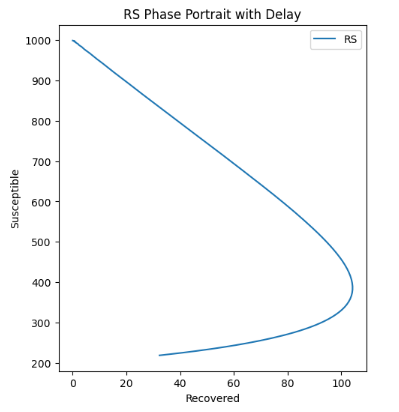
\includegraphics[width=\textwidth]{SR-2.png}
\caption{Phase portrait for the $S$ and $R$ compartments.}
\end{minipage}
\hfill
\begin{minipage}[b]{0.23\textwidth}
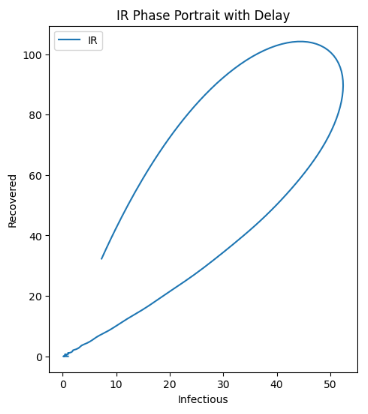
\includegraphics[width=\textwidth]{IR-2.png}
\caption{Phase portrait for the $I$ and $R$ compartments.}
\end{minipage}
\hfill
\begin{minipage}[b]{0.23\textwidth}
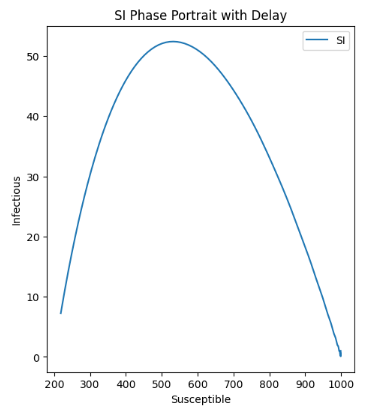
\includegraphics[width=\textwidth]{SI-2.png}
\caption{Phase portrait for the $I$ and $S$ compartments.}
\end{minipage}
\end{figure}
To obtain the phase portrait, we can use the Python package matplotlib to plot the vector field of the system of differential equations.

\section{Solution Curve}
To obtain the solution curve of the SIR model, we can use the Python package scipy to numerically integrate the system of differential equations using the function odeint. We can specify the initial values of $S$, $I$, and $R$, the values of $\beta$ and $\gamma$, and the time range over which we want to obtain the solution.
\begin{figure}[htbp]
\centering
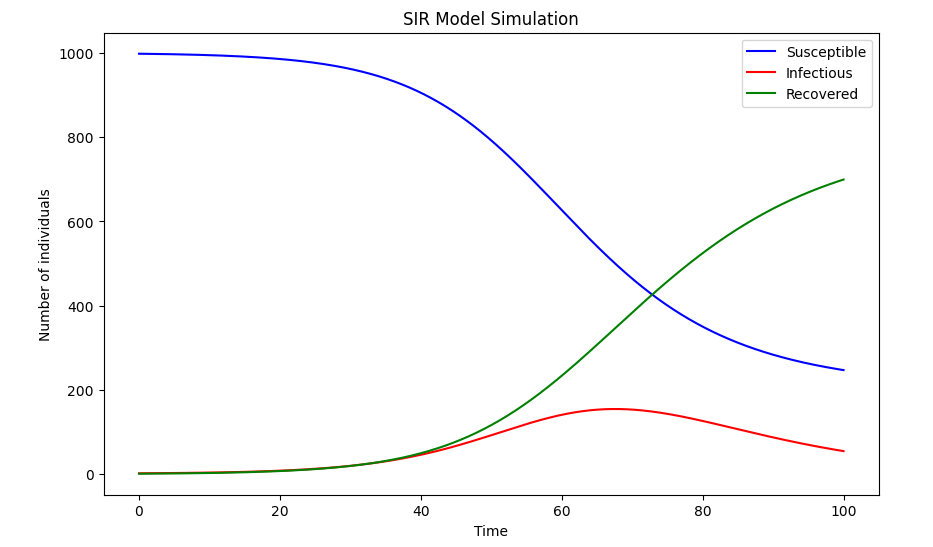
\includegraphics[width=0.65\textwidth]{solution-curve.png}
\caption{Solution Curve}
\label{fig:architecture}
\end{figure}
\\

\item[(c)] Comparing the two models, The two models, the SIR model with delay and the original SIR model without delay, capture different aspects of disease transmission dynamics.
\\
The SIR model with delay incorporates the delay in the response of the infected population to the infection, which could be due to a lag in testing or the incubation period of the disease. This delay results in a slower growth rate of the infected population and a delayed peak in the number of infections. The delay can be beneficial in situations where the response time of the infected population is significant, and the health system can't handle a sudden increase in the number of cases.
\\
On the other hand, the original SIR model without delay assumes that the infected population responds immediately to the infection. The model's predictions are more optimistic than those of the SIR model with delay, and the model's results are often used as a benchmark for comparison with other models. However, the model's assumptions may not hold in real-world scenarios, where the response time of the infected population is not instantaneous.\\

 If the response time of the infected population is significant, and the health system can't handle a sudden increase in the number of cases, then the SIR model with delay would be more appropriate. On the other hand, if the response time of the infected population is not significant and the health system can handle a sudden increase in the number of cases, then the original SIR model without delay may be more appropriate.
\\
In the current scenario of the COVID-19 pandemic, where there is a high risk of overwhelming the healthcare system with a sudden increase in the number of cases, the SIR model with delay may be more beneficial. The delayed response of the infected population to the infection, due to the lag in testing or incubation period, is a critical factor in the spread of COVID-19. Therefore, the SIR model with delay can provide a more accurate estimation of the peak of the epidemic and the timing of the response of the healthcare system.

\end{enumerate}

\section{Conclusion}
In this report, we have simulated the SIR model using Python and obtained the phase portrait and solution curve of the system. The SIR model is a simple and useful tool for understanding the dynamics of infectious diseases in a population. However, the model has limitations and its results should be interpreted with caution. Further research is needed to improve the accuracy and applicability of the SIR model and to develop more sophisticated models that take into account the complexities of real-world populations.
\bibliography{reference}
\bibliographystyle{plain}
\cite{kermack1927contribution,brauer2017mathematical,hethcote2000mathematics,allen2007introduction,keeling2008modeling}
\end{document}


